\subsection{Hivatkozások}

%_
\begin{frame}
  A \emph{látszólagos osztály} (pseudo class) egy, a szelektor utáni 
  :-ot követő kulcsszó, amivel a kiválasztott elem(ek) különféle 
  állapotaiban alkalmazandó formázás adható meg.\\
  \vfill
  \hiv{\href{https://developer.mozilla.org/en-US/docs/Web/CSS/Pseudo-classes}{Látszólagos osztályok referenciája}}
  \vfill
  Hivatkozásoknál alkalmazható:
  \begin{description}[m]
    \item[\texttt{link}] \hfill \\ Még nem követték a hivatkozást
    \item[\texttt{visited}] \hfill \\ Már követték a hivatkozást
    \item[\texttt{hover}] \hfill \\ Egér a hivatkozás felett
    \item[\texttt{active}] \hfill \\ Már rákattintottak, de az új 
    tartalom még nem töltődött be
  \end{description}
  \kiemel{Ebben a sorrendben} kell definiálni őket!
\end{frame}

%
\begin{frame}
  \begin{exampleblock}{\textattachfile{hivatkozas.html}{hivatkozas.html}}
    \scriptsize
    \lstinputlisting[style=HTML,linerange={7-10},numbers=left,firstnumber=7]{hivatkozas.html}
    \lstinputlisting[style=HTML,linerange={14-16},numbers=left,firstnumber=14]{hivatkozas.html}
  \end{exampleblock}
  \begin{center}
    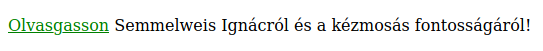
\includegraphics[width=0.8\textwidth]{hivatkozas.png}
  \end{center}
\end{frame}
